    % je commente, car je ris à chaque fois que je lis cette ligne :
%   PARLER DES DUDES QU'ON A RENCONTRE A PERLARONIE
Ce projet, d'un choix assumé par les étudiants et la société NaturalPad qui en est l'inspiratrice, comporte 
une composante recherche forte. C'est dans cette optique et comme expliqué en \ref{etude_terrain} que nous avons 
commencé notre projet par un travail d'investigation et de recherche d'informations. Dans ce but, nous avons rencontré 
des praticiens de l'hôpital Lapeyronie à Montpellier : Julien Métrot, doctorant du Laboratoire Movement To Health et 
Karima Bakhti, kinésithérapeute au CHU de Montpellier. Lors de cette entrevue, ils ont partagé avec nous leurs 
connaissances sur le test de Fugl Meyer et bien plus encore, et nous ont offert la possibilité d'assister à la 
réalisation d'un tel test sur une patiente atteinte d'hémiplégie.
  \section{Fugl Meyer}\label{fugl_meyer}
Le test de Fugl Meyer constitue un ensemble d'exercices à effectuer par le patient, et dont chaque mouvement est 
évalué selon un ou plusieurs critères, fournissant un score généralement compris entre 0 [échec], 1 [intermédiaire]
et 2 [réussite]. Ces exercices peuvent concerner successivement les membres inférieurs et supérieurs, eux même divisés 
en sous catégories. Pour les membres supérieurs, on notera la présence d'un score \textit{proximal}
\footnote{une partie du corps proche de la racine d'un membre} et d'un score
\textit{distal}\footnote{partie d'un membre la plus éloignée de la base de celui-ci.}. 
Ce test a pour vocation d'être réalisé régulièrement tout au long de la période de réhabilitation
du patient, afin de mesurer ses progrès.
  \section{Réalisation du test}
        \subsection{Contexte}
Nous avons assisté à la passation d'un test de FM sur une jeune patiente atteinte d'une hémiplégie suite à un AVC ; 
ses membres supérieurs droits étaient affectés. Comme nous l'ont précisé J. Métrot et K. Bahkti, seules les parties 
du test concernant les membres supérieurs ont donc bien sur été réalisées. Pour les détails des mesures et exercices 
effectués lors de ce test, se référer à l'annexe \ref{evaluation_FM}.

\begin{figure}[h!]
\centering
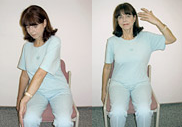
\includegraphics[width=0.5\linewidth]{images/fuglmeyer_example}
\caption{Exemple d'un exercice du membre supérieur du test de Fugl-Meyer.}
\end{figure}

        \subsection{À noter}
Les patients concernés par la rééducation des membres supérieurs, comme la patiente qui a accepté de passer 
le FM en notre présence, sont globalement plus nombreux. Cela concorde avec les contraintes du capteur Kinect, 
qui possède un petit angle de vue. Il est alors nécessaire d'avoir beaucoup d'espace (de recul) dès lors que 
l'on souhaite capter l'intégralité d'une personne de manière précise. \\
Lors des tests, le médecin ou personnel médical s'occupant du patient, peut être amené à 'aider' celui-ci.
Cela peut se traduire, outre les éventuels encouragements oraux, en maintenant ou en bloquant un membre du patient
non directement concerné par l'exercice du test. Par exemple, lorsque l'on demande au patient de "tourner son avant 
bras" (prono-supination de l'avant bras) avec le bras tendu, le praticien peut aider le patient à maintenir son bras
(partie haute).\\
Notons aussi qu'en l'occurrence, les praticiens n'ont pas eu besoin d'utiliser de goniomètre ou autre instrument de 
mesure pour évaluer la qualité des gestes de la patiente.
    
  \section{L'avis des professionnels}
  Le test de Fugl Meyer est le plus répandu et accepté : il constitue le "gold standard" dans le milieu.
  Nos interlocuteurs regretteront toutefois une certaine subjectivité et interprétation des résultats.
  Nous en avons d'ailleurs eu une démonstration lors de ce test : il arrivait que K. Bahkti et J. Métrot 
  évaluent différemment les mouvements de la patiente. \\
Une autre critique est "l'effet plateau" qu'induit ce test. En effet, l'échelle de mesure est très petite 
(2, maximum 3 valeurs de notation) et le patient atteindra régulièrement des 'seuils' sur son score global. 
C'est-à-dire que même si il réalise encore des progrès par rapport aux fois précédentes, cela ne sera pas forcément 
visible et impactant sur le score global, à cause du manque de granularité de la mesure. Même si cela n'est pas une 
fin en soi, on peut noter l'aspect peu encourageant que cela peut apporter au patient. \\
Pour les mêmes raisons, le patient pourra obtenir un score maximal (dans notre étude de cas, 66/66) sans pour autant
avoir recouvré la totalité de ses capacités, et quand bien même des progrès sont encore possibles. \\
Cela amène au regret que le test standard soit un test jugeant la \textbf{déficience} et non la \textbf{fonctionnalité}. 
Il existe cependant de nombreux autres tests, et une des alternatives intéressantes est le test "ARAT : 
Action Research Arm Test". %TODO réf lien
Rapidement, ce test consiste à vérifier si un patient est capable d'effectuer un geste du quotidien (déplacer
un objet, se servir un verre d'eau, etc), et de chronométrer le temps que cela lui a pris. C'est donc un test 
de fonctionnalité.
  
  \subsection{Impressions et propositions}
Après notre entretien et cette passation du test de FM, et à partir de nos tests préliminaires, nous en avons 
conclu que l'utilisation du kinect semblerait plus adaptée pour faire une évaluation des performances \textbf{proximales}.
En effet, la taille des membres et l'amplitude des gestes requis pour l'évaluation proximale offrent de bien 
meilleures possibilités d'analyse des mouvements. Certains gestes du poignet sembleraient aussi bien adaptés.
\paragraph{}En revanche, les autres mouvements distaux semblent trop difficiles à percevoir et à interpréter par le capteur.
L’idée serait de proposer une évaluation de grain plus fine, allant au delà d’une évaluation ternaire entre 
“a réussi à lever le bras à l’horizontal”, “a levé son bras partiellement” et “n’a pas réussi à lever son bras”. 
Il serait utile de pouvoir donner l’angle exact, par exemple.   

\paragraph{}Les tests sur la main sont évalués de manière “tactile” (tests de résistance, de préhension) pour la plupart, 
avec peu de différence visuelle entre une évaluation 0 et 2. L’utilisation de la Kinect semble alors peu pertinente
pour cette partie de l’évaluation.
